\section*{\hypertarget{char}{Characters}}
\addcontentsline{toc}{section}{Characters}
%
"I am THE Basch fon Ronsenburg!" \\
\indent -- Vaan
%
\begin{center} 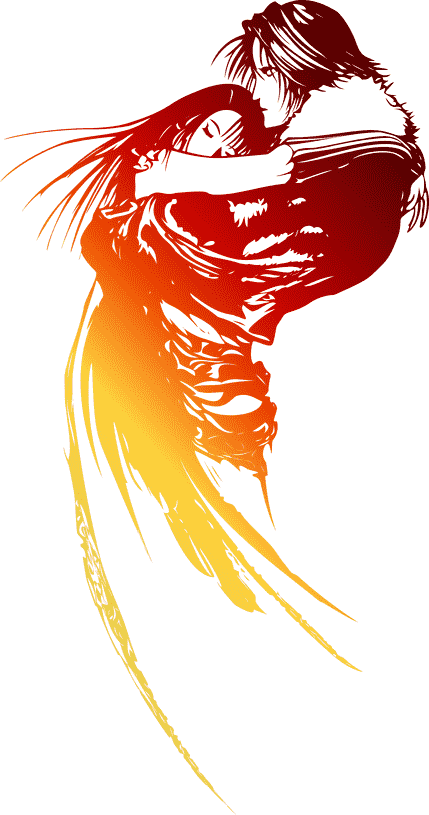
\includegraphics[width=0.9\columnwidth]{./art/images/ff8.png} \end{center}
%
All players play as one of the adventurers in the party of protagonists. 
They immerse themselves into their character and talk and act from their perspective. 
The GM also creates and takes the role of many non-player characters throughout the adventure.
All these characters inhabit the world created by the GM and shape it through their actions and decisions.
This section details different aspects that describe a character. 

\subsubsection*{Character Creation}
Characters usually have distinct appearances, personalities, strengths and weaknesses. 
Therefore, the character creation rules present many opportunities to customize how characters feel and play.
The following guide walks you through all necessary steps to create your character.
\pagebreak%

\begin{enumerate}[leftmargin=*]
	
\item Copy or print out the \hyperlink{cs}{Character Sheet} that is included on the next page.
The sheet helps you to keep track of important information about your character which you can fill in while following this section.
There is also an \hyperlink{csex}{example} of a filled out sheet, which you can use as a guideline to fill out yours.

\vfill 

\item Choose your character's name and give a short \textbf{Description} of him or her.
Here, you should also communicate with your GM so you can integrate your character better into the game world.
For example if different races or tribes exist in the world, your character may be part of one of them.

\vfill	

\item Briefly summarize your character's \textbf{Story} until now and explain his or her motivation for joining the party on this adventure.
Consider that this is most likely your character's first serious adventure, so he or she probably does not have significantly more experience than the average person.

\vfill

\item Choose your character's \textbf{Talent}, which grant special proficiencies in a non-combat skill.
Read the \mbox{\hyperlink{talent}{Talents subsection}} for more details.

\vfill

\item Choose your character's \textbf{Job} which determine combat related proficiencies. 
Characters usually start the game at Level~1, where their starting attributes and abilities are determined by the chosen Job.
Read the \hyperlink{job}{Jobs~subsection} for more details.

\vfill

\item Depending on the chosen job, your character gains expertise in certain classes of weapons and armor.
Discuss with your GM which specific starting \textbf{Equipment} makes sense for your character.
Read the \hyperlink{equip}{Equipment subsection} for more details.

\end{enumerate}

\vspace{1cm}

\example{Character Creation}
{
We create a character named "Vaan", who is a 17-year old, blonde-haired human boy with athletic appearance. 
Vaan is an orphan, who gets by in the big city by stealing from the townsfolk and often acts as a father figure to other orphans.
He dreams of owning an airship and being a sky pirate one day. 
First, we check with the GM that Vaan fits well enough with the given setting and the rest of the party.
Then, we choose the \hyperlink{talent}{Leading Man} talent and the \hyperlink{Thief}{Thief} job, which seem to fit Vaan best.
From the Basic Attributes table of the job we determine Vaan's maximum HP~(20), maximum MP~(14) and AGI (4), all other attributes start at 0.
We also note that he learns the "Steal Gil" tech.
Finally, we decide with the GM that it makes sense that our poor thief has a \hyperlink{mknife}{Mythril Knife}, Clothes and 100 Gil as his starting equipment.
}

\pagebreak
